\section{Workflow Overview} % (fold)
\label{sec:workflow_overview}

This section provides a brief overview of how MiCS works. Figure \ref{fig:mics_internal_workflow} shows the five stages that MiCS goes through when converting C\# to JavaScript.

Basically, MiCS uses Roslyn to generate an AST representing the user’s C\# code. This AST is validated and mapped to a Script\# AST, that represents JavaScript. From the Script\# AST, JavaScript is generated and finally injected into the user’s WebForm page.

\begin{figure}[H]
	\begin{center}
		\centerline{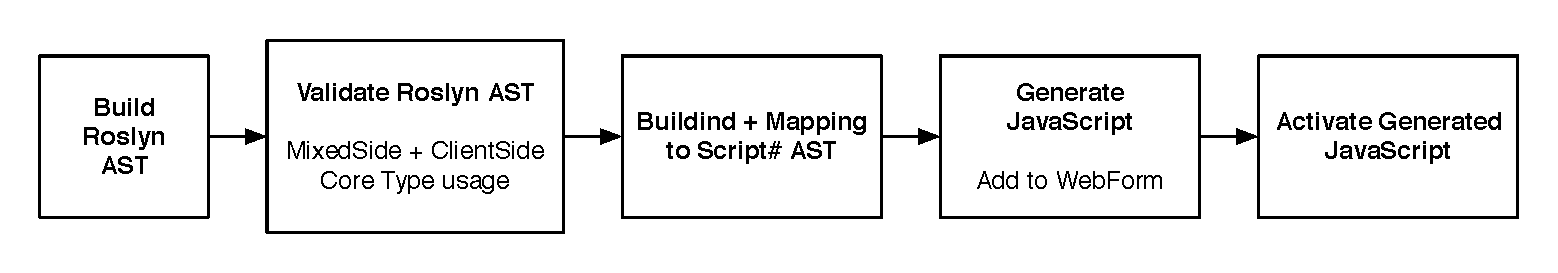
\includegraphics[width=14cm]{resources/images/internalworkflow.eps}}
	\end{center}
	\caption{The MiCS internal workflow}
	\label{fig:mics_internal_workflow}
\end{figure}

MiCS uses Roslyn to generate an Abstract Syntax Tree which is a syntatic representation of the user’s C\# code. Apart from the AST, a Semantic Model is generated to obtain information about what is being referenced.

When the Roslyn AST has been obtained it needs to be validated. This is done to ensure that the user uses types in a correct manner. Without validation, it would be possible for the user to generate non-working JavaScript.

Once the syntax tree has been validated, it is ready to be mapped to Script\#. This is the core functionality of MiCS - transforming a Roslyn AST to a Script\# AST. This step also ensures that the user does not utilize C\# constructs (declarations, statements and expressions) that we do not support. For example, at the moment the only supported loop-type is the for-loop. So if the user uses a while-loop or a foreach loop, the user gets an error telling them that an unsupported construct has been used.

When the Roslyn AST has successfully been mapped to Script\#, MiCS uses Script\#’s built-in ScriptGenerator to generate the JavaScript corresponding to the user’s original C\# code. 

When the JavaScript has been generated, it needs to be injected into the users WebForm. This is handled by a MiCSPage class; an extension to a WebForm Page. 

% section workflow_overview (end)